%%%%%%%%%%%%%%%%%%%%%%%%%%%%%%%%%%%%%%%%%%%%%%%%%%%%%%%%%%%%%%%%%
% Projeto de Extensão da disciplina de Matemática Discreta
% Sub-projeto do ProgramAuto
% Autores:
%     Prof. Dr. Ruben Carlo Benante
%     Nome do Aluno Alex Bruno Seabra
%     Nome do Aluno 2
%
% Data: 2021-06-14
%
% Assunto: escrever uma linha de explicação
%%%%%%%%%%%%%%%%%%%%%%%%%%%%%%%%%%%%%%%%%%%%%%%%%%%%%%%%%%%%%%%%%


%%%%%%%%%%%%%%%%%%%%%%%%%%%%%%%%%%%%%%%%%%%%%%%%%%%%%%%%%%%%%%%%%
% Para gerar o PDF use uma das 2 opções abaixo:
%
% Opção 1: com makefile
%    $ make ext-matdiscreta-benante-sobrenome1-sobrenome2.pdf
%
% Opção 2: comandos diretos:
%    $ pdflatex pext-matdiscreta-benante-sobrenome1-sobrenome2.tex -o pext-matdiscreta-benante-sobrenome1-sobrenome2.pdf
%    $ bibtex biblio 
%    $ pdflatex pext-matdiscreta-benante-sobrenome1-sobrenome2.tex -o pext-matdiscreta-benante-sobrenome1-sobrenome2.pdf

% preambulo %%%%%%%%%%%%%%%%%%%%%%%%%%%%%%%%%%%%%%%%%%%%%%%%%%%%%%
\documentclass[a4paper,10pt]{article} %twocolumn
\usepackage[utf8]{inputenc} % letras acentuadas
\usepackage[portuguese]{babel} % tradução de títulos
\usepackage{algorithm} % ambiente para índice de algoritmos
\usepackage{algpseudocode} % fonte e estilo do algoritmo
\usepackage{graphicx}
% \usepackage{natbib}
%[noend]

\floatname{algorithm}{Algoritmo} % tradução da palavra algorítimo no ambiente de índice

% capa %%%%%%%%%%%%%%%%%%%%%%%%%%%%%%%%%%%%%%%%%%%%%%%%%%%%%%
\title{ProgramAuto: biblioteca Ncurses}
\author{Ruben Carlo Benante \\ Alex Bruno Seabra \\ Autor3}  % nome dos outros alunos

\begin{document}

\maketitle

% resumo %%%%%%%%%%%%%%%%%%%%%%%%%%%%%%%%%%%%%%%%%%%%%%%%%%%%%%
\begin{abstract}

\textbf{Assunto:} Ensino da Linguagem de Programação \texttt{C}.
Vamos abordar a biblioteca Ncurses e explicar o funcionamento do projeto de extensão
% descrever em poucas palavras seu projeto aqui 

\textbf{Local:} Escola Politécnica de Pernambuco - UPE/POLI

\textbf{Órgão Financiador:} N/A

\textbf{Caracterização:} Projeto de Extensão requisito da disciplina de Matemática Discreta, sub-projeto integrante do Projeto \texttt{ProgramAuto}

% Este é o fim do resumo.

\end{abstract}


% artigo %%%%%%%%%%%%%%%%%%%%%%%%%%%%%%%%%%%%%%%%%%%%%%%%%%%%%%
% seção de introdução %%%%%%%%%%%%%%%%%%%%%%%%%%%%%%%%%%%%%%%%%%%%%%%%%%%%%%
\section{Introdução}

% Descrever melhor seu projeto aqui 

O projeto de extensão vai ser um minicurso sobre a biblioteca Ncurses em liguagem C. Neste curso serão abordados algumas 
das pricipais  funções dessa biblioteca bem como algumas de suas aplicações.

% seção de objetivos %%%%%%%%%%%%%%%%%%%%%%%%%%%%%%%%%%%%%%%%%%%%%%%%%%%%%%
\section{Objetivos}

\subsection{Objetivo Geral}
O projeto tem como objetivo principal contribuir paraa melhorar o ensino dos discentes interessados promovendo ações para capacitação da comunidade a fim de colaborar com o desenvolvimento técnico cientifico.

\subsection{Objetivos Específicos}

Listar os objetivos específicos

\begin{itemize}
 \item Proporcionar tal e tal
 \item Realizar tal e tal
\end{itemize}


% seção de justificativa %%%%%%%%%%%%%%%%%%%%%%%%%%%%%%%%%%%%%%%%%%%%%%%%%%%%%%
\section{Justificativa}



\begin{figure}[!htb]
\centering
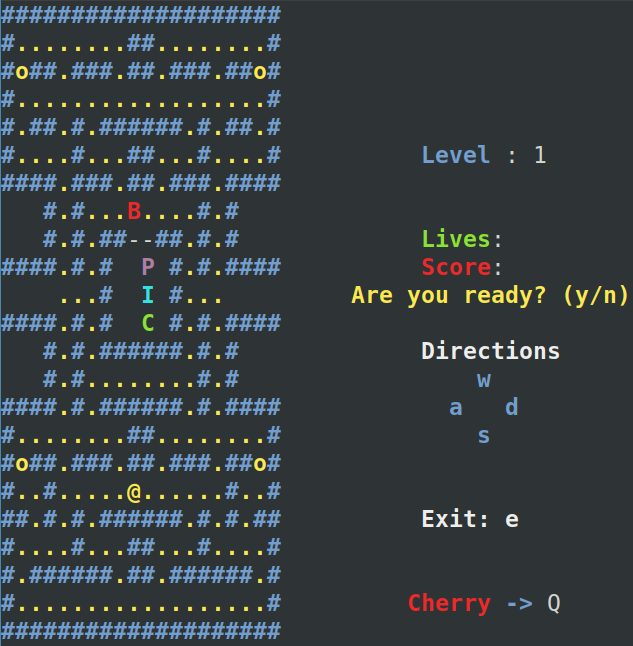
\includegraphics[width=.80\linewidth]{imagem.png}
\caption{Exemplo de aplicação do Ncurses.}
\label{fig:xsort}
\end{figure}


% seção de metodologia %%%%%%%%%%%%%%%%%%%%%%%%%%%%%%%%%%%%%%%%%%%%%%%%%%%%%%
\section{Metodologia}

Descrever como (por quais métodos) os objetivos serão alcançados.

O algoritmo é descrito abaixo:

% subseção equipamentos %%%%%%%%%%%%%%%%%%%%%%%%%%%%%%%%%%%%%%%%%%%%%%%%%%%%%%
\subsection{Equipamentos Necessários}
Programas de edição de video

%Listar os equipamentos necessários para a implementação do projeto.

Para realizar este projeto é preciso tal e tal

O método \emph{Ysort} é caracterizado por...

% subseção com algoritmo %%%%%%%%%%%%%%%%%%%%%%%%%%%%%%%%%%%%%%%%%%%%%%%%%%%%%%
\subsection{Implementação}

A implementação será feita por meio de uma pequena playlist no youtube


%\begin{algorithm}
%\caption{Algoritmo Ysort}\label{alg:ysort}
%\begin{algorithmic}[1]
%\Function{ysort}{estado}\Comment{retorna uma ação}
%\State \textbf{Entradas}: estado é a configuração atual do jogo
%\State $v\gets \mathrm{maxvalor}{(estado)}$
%\State \textbf{returna} a ação $a$ em sucessores(estado) cujo valor é $v$ %\Comment{comentario}


% \While{$r\not=0$}\Comment{We have the answer if r is 0}
% \State $a\gets b$
% \State $b\gets r$
% \State $r\gets a\bmod b$
% \EndWhile\label{euclidendwhile}


%\EndFunction
%\Function{maxvalor}{estado}\Comment{retorna o valor estático}
%\If{fim(estado)}
%   \State \textbf{retorna} estatico(estado)
%\EndIf
%\State $v \gets -\infty$
%\For{todas ações $a$ nos sucessores(estado)}
%    \State $v \gets \max{(v, \mathrm{minvalor}(a))}$
%\EndFor
%\State \textbf{retorna} $v$
%\EndFunction
%\Function{minvalor}{estado}\Comment{retorna o valor estático}
%\If{fim(estado)}
%   \State \textbf{retorna} estatico(estado)
%\EndIf
%\State $v \gets \infty$
%\For{todas ações $a$ nos sucessores(estado)}
%    \State $v \gets \min{(v, \mathrm{maxvalor}(a))}$
%\EndFor
%\State \textbf{retorna} $v$
%\EndFunction
%\end{algorithmic}
%\end{algorithm}




% seção Plano de Trabalho %%%%%%%%%%%%%%%%%%%%%%%%%%%%%%%%%%%%%%%%%%%%%%%%%%%%%%
\section{Plano de Trabalho}

 \begin{itemize}
  \item Pesquisa do conteudo
  \item implementação dos códigos que serão usados para exemplificação
  \item roteiro dos videos
  \item editar os videos 
 \end{itemize}


% seção Plano de Trabalho %%%%%%%%%%%%%%%%%%%%%%%%%%%%%%%%%%%%%%%%%%%%%%%%%%%%%%
\section{Cronograma}

Em conjunto com a seção de Plano de Trabalho, a seção de cronograma coloca as atividades dispostas numa linha do tempo.

Utilize uma tabela para melhor visualização.

\begin{table}
\begin{center}
 \caption{Tabela de cronograma do projeto de extensão}
\begin{tabular}{|l|r|}
  \hline \hline
  \textbf{Etapas} & \textbf{Datas} \\ \hline \hline
  Pesquisa do conteudo & 24/06 \\ \hline
  implementação dos códigos & 03/07 \\ \hline
  roteiro dos videos & 11/07 \\ \hline
  editar os videos & 15/07 \\ \hline \hline
\end{tabular} 
\label{tab:resultados}
\end{center}
\end{table}


% seção de impactos alcançados %%%%%%%%%%%%%%%%%%%%%%%%%%%%%%%%%%%%%%%%%%%%%%%%%%%%%%
\section{Impactos e Transferências}

% subseção de impacto científico %%%%%%%%%%%%%%%%%%%%%%%%%%%%%%%%%%%%%%%%%%%%%%%%%%%%%%
\subsection{Impacto Científico}

Não há impacto científico relevante.

% subseção de impacto tecnológico %%%%%%%%%%%%%%%%%%%%%%%%%%%%%%%%%%%%%%%%%%%%%%%%%%%%%%
\subsection{Impacto Tecnológico}

Não há impacto tecnológico relevante.

% subseção de econônimo %%%%%%%%%%%%%%%%%%%%%%%%%%%%%%%%%%%%%%%%%%%%%%%%%%%%%%
\subsection{Impacto Econômico}

Não há impacto econômico relevante.

% subseção de impacto social %%%%%%%%%%%%%%%%%%%%%%%%%%%%%%%%%%%%%%%%%%%%%%%%%%%%%%
\subsection{Impacto Social}

O projeto visa contribuir com a sociedade transmitindo conhecimento gratuito aberto a todas as pessoas
no youtube

% subseção de impacto ambiental %%%%%%%%%%%%%%%%%%%%%%%%%%%%%%%%%%%%%%%%%%%%%%%%%%%%%%
\subsection{Impacto Ambiental}

Não há impacto ambiental relevante.

% subseção de transferências %%%%%%%%%%%%%%%%%%%%%%%%%%%%%%%%%%%%%%%%%%%%%%%%%%%%%%
\subsection{Transferências}

O ProgramAuto terá como objetivo a execução de aulas para ensinar a linguagem C aos discentes interessados. Contará com sua exposição de ensino gravada que será disponibilizada e a elaboração de relatórios a fim de cumprir com os aspectos estabelecidos no Plano de Trabalho. O projeto transfere conhecimento para todas as pessoas de forma gratuita a fim de colaborar com a sociedade no seu desenvolvimento cultural e intelectual.


% seção de resultados esperados %%%%%%%%%%%%%%%%%%%%%%%%%%%%%%%%%%%%%%%%%%%%%%%%%%%%%%
\section{Resultados Esperados}

Os resultados mostrados na tabela \ref{tab:resultados} demonstram ...

    Concluimos,com base nos estudos e testes coletados sobre os algoritmos de ordenação propostos, que para fins educacionais, o algoritmo \textit{BubbleSort} é mais indicado devido a sua simples implementação, cabendo então para o \textit{QuickSort} ser o mais indicado entre os dois, quando requer uma demanda em menor tempo e com mais eficiência.

De acordo com \cite{Benante2008phd}, este é o fim do artigo.

%%%%%%%%%%%%%%%%%%%%%%%%%%%%%%%%%%%%%%%%%%%%%%%%%%%%%%%%%%%%%%%%%%%%%%%%%%%%%%%%%%%%%%%%%%%%%%%%%%%%%%%%%%%%
% referências bibliográficas %%%%%%%%%%%%%%%%%%%%%%%%%%%%%%%%%%%%%%%%%%%%%%%%%%%%%%
%\section*{Referências Bibliográficas}

% cite todos, mesmo os não referenciados %%%%%%%%%%%%%%%%%%%%%%%%%%%%%%%%%%%%%%%%%%%%%%%%%%%%%%
\nocite{*}

% se necessario %%%%%%%%%%%%%%%%%%%%%%%%%%%%%%%%%%%%%%%%%%%%%%%%%%%%%%
% troca autor and autor por autor & autor, na bibliografia. O dcu usa "and"
%\renewcommand{\harvardand}{\&} % troca and pro &. O dcu usa "and"

% Estilos de bibliografia %%%%%%%%%%%%%%%%%%%%%%%%%%%%%%%%%%%%%%%%%%%%%%%%%%%%%%
% \bibliographystyle{abnt-alf} % Estilo alfabético da ABNT. Opção [num] para estilo numérico
%\bibliographystyle{apalike}
%\bibliographystyle{dcu} %citacao como (autor and autor, ano). Parece apalike. Rev. Control. Automacao. Use com harvard
%\bibliographystyle{agsm} % padrao harvard fica (autor & autor ano).
\bibliographystyle{acm}

% arquivo de banco de dados das referências %%%%%%%%%%%%%%%%%%%%%%%%%%%%%%%%%%%%%%%%%%%%%%%%%%%%%%
% renomear para o número do exercício correto
% o arquivo de bibliografia pode se chamar qualquer coisa, isso não muda o comando de gerar o PDF. 
% Por exemplo para 'mybiblio.bib', use \bibliography{mybiblio} e os comandos pdflatex e bibtex continuam os mesmos identicos com exN.
\bibliography{biblio}

\end{document}
